\section{Tutorial}\label{Tutorial}

The tutorial describes few main cases of the arbitrary user, neural network engineer and contributor user. The use cases will be described in UML  Activity Diagram. The details will be skipped, only the main function will be described.  

\subsection{Using Network and Model Repositories}\label{Using Network and Model Repositories}

The arbitrary user does not have a lot of experience in neural network field. In the most cases, he wants just to get into the subject by learning on the N2Sky platform. 

\begin{figure}[htbp]
\begin{center}
  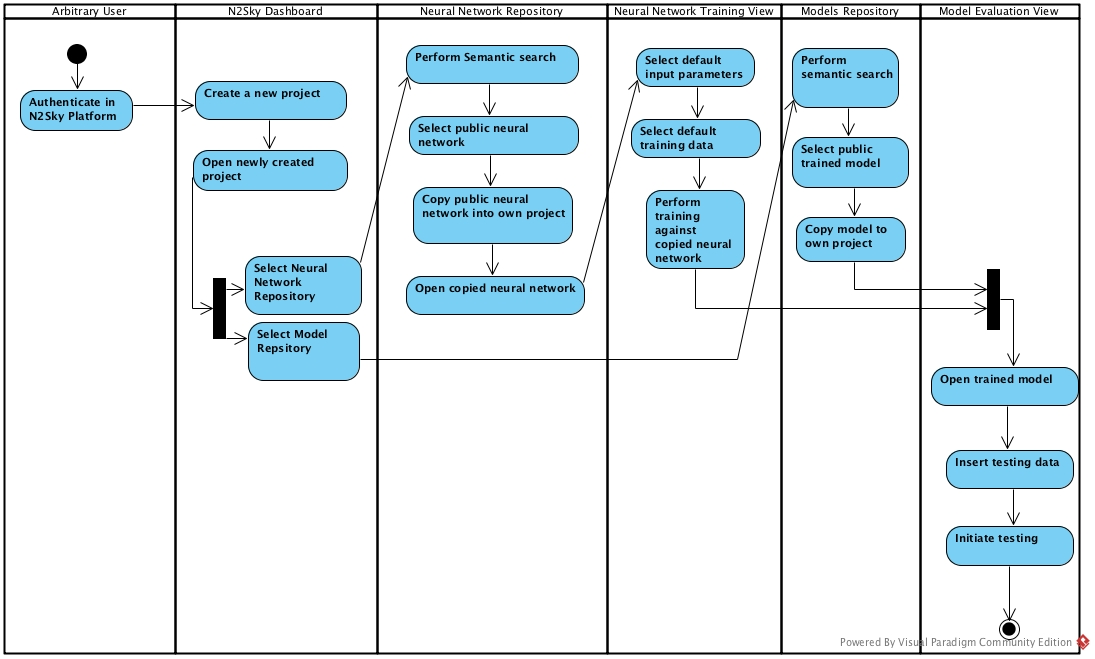
\includegraphics[width=\linewidth]{components/tutorial/img/training_arbitrary.jpg}
  \caption{Tutorial. Activity Diagram of using Network and Model Repositories}
  \label{fig:training_arbitrary}
\end{center}
\end{figure} 

The activity diagram, which displayed in figure \ref{fig:training_arbitrary}, shows typical workflow of using the neural network and models repositories. There are six main components of the diagram, which are participating in this workflow: 
\begin{enumerate}
\item The arbitrary user
\item N2Sky Dashboard
\item Neural Network Repository
\item Neural Network Training View
\item Models Repository
\item Model Evaluation View
\end{enumerate}

Every participant is represented as a pool of activities. The following steps the user has to proceed:

\begin{itemize}
\item \emph{The arbitrary user} 
\begin{itemize}
\item \emph{Authenticate in N2Sky platform} is the first step for every user, which starts to use the N2Sky platform. 
The user has to either log in with existing credentials or signup on start page as is shown in figure \ref{fig:sign_login}

\begin{figure}[H]
\begin{center}
  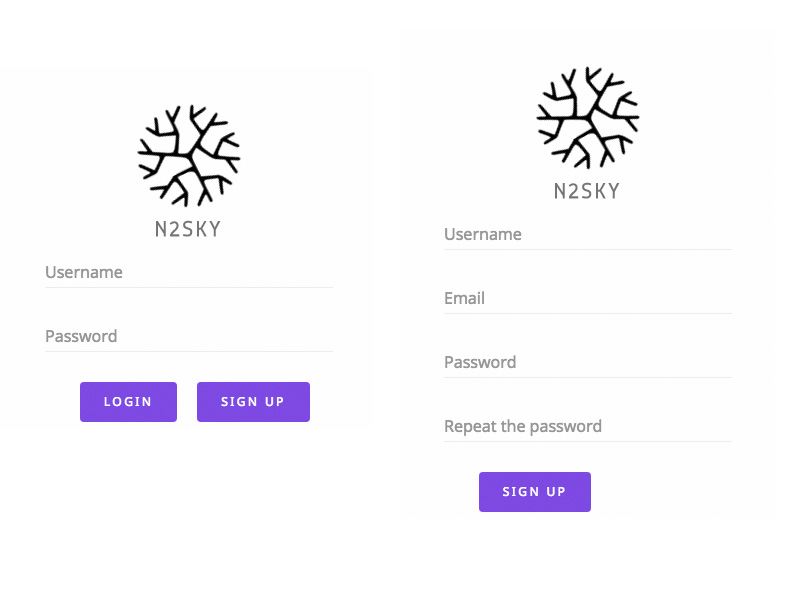
\includegraphics[width=\linewidth]{components/tutorial/img/sign_login.jpg}
  \caption{Tutorial. Login form on the left sight and the signup form on the right.}
  \label{fig:sign_login}
\end{center}
\end{figure} 
\end{itemize}
\item \emph{N2Sky Dashboard} 
\begin{itemize}
\item \emph{Create a new project.} The user goes to own dashboard and clicks on "Create project" button. The popup modal window will appear and the user can type the name of the project and the short description. After the project is created it will authenticly appear on the dashboard of the user.  
\item \emph{Open newly created project} by clicking on the folder with the newly created project name.
\item \emph{Select Neural Network Repository.} When the user will be in the project view he will see the list of the tools in the top bar. One of the tools is "Neural network repository". By clicking on it the user will be redirected to Neural Network Repository page.
\end{itemize}
\item \emph{Neural Network Repository}
\begin{itemize}
\item \emph{Perform Semantic Search.} The user will see on the top bar of the page the searching fields with filters. The user can perform the semantic search in order to find the desirable neural network. 
\item \emph{Select public neural network.} The arbitrary user can select publicly available neural network. He can observe the details of the neural network.
\item \emph{Copy public neural network into own project.} If the user satisfied with the selected neural network he can copy it into own project. The copy button is located right on the neural network and it looks like a star button. On click, the popup window will appear and the user can select his project.
\item \emph{Open copied neural network.} After copying the neural network user can up it and perform some training. The arbitrary user does not have permission to see how other people used the neural network.
\end{itemize}

\item \emph{Neural Network Training View}. This view is the part of the "3-steps-view" of creation of the neural network from paradigm. For arbitrary user, all other views are available only in read-only mode.
\begin{itemize}
\item \emph{Select default input parameters.} Since the arbitrary user does not have experience, he is always going with default values in every form.
\item \emph{Select default training data.} The same default possibilities chose the arbitrary user just by clicking "User default values".
\item \emph{Perform training against copied neural network.} After selecting all default values, the user can click on "Perform Training" button. The training status will appear in the table below.
\end{itemize}

\item \emph{Models Repository.} This is second possibility of the arbitrary user if he choose the "Model Repository" tool from his own project in N2Sky Dashboard.
\begin{itemize}
\item \emph{Perform Semantic Search.} The user will see on the top bar of the page the searching fields with filters. The user can perform the semantic search in order to find desirable trained model.
\item \emph{Select trained model.} The user can select and observe trained model before copying it.
\item \emph{Copy model into the own project} by clicking on "Copy" button. The popup modal window will appear and the user can choose his project.
\end{itemize}

\item \emph{Model Evaluation View.} This step merge selection of the neural network with performed trained model and selection of the existing trained model because the next activities are the same for both cases.
\begin{itemize}
\item \emph{Open trained model.} The use clock on the trained model and the detailed information with a training data will appear.
\item \emph{Insert testing data.} The user clicks on "Test model" button and the popup window will appear. The arbitrary user uses default testing data without changing it.
\item \emph{Initiate testing.} After proceeding the testing, the evaluation information will appear in the table. The user can study the data and check if the testing results are correct.
\end{itemize}


\end{itemize}



\subsection{Creation of the Neural Network from the Existing Paradigm}\label{Creation of the neural network from the existing paradigm}

This case is related to neural network engineer user. Some steps are familiar to the previous case with the arbitrary user, but mostly the user of the platform is different. The arbitrary user wanted to use everywhere default data and copy existing neural networks and model. The neural network engineer user already experiences user and he can create his own neural network from existing paradigm and perform training and testing with his own data.


The activity diagram, which displayed in figure \ref{fig:tutorial_engeneer}, shows typical workflow of creating the neural network from existing paradigm. There are four main components of the diagram, which are participating in this workflow: 
\begin{enumerate}
\item The neural network engineer user
\item N2Sky Dashboard
\item "3-step-view" with sub-components:
\begin{itemize}
\item Neural network description
\item Neural network structure
\item Neural network training
\end{itemize}
\item Model Evaluation View
\end{enumerate}

\begin{figure}[H]
\begin{center}
  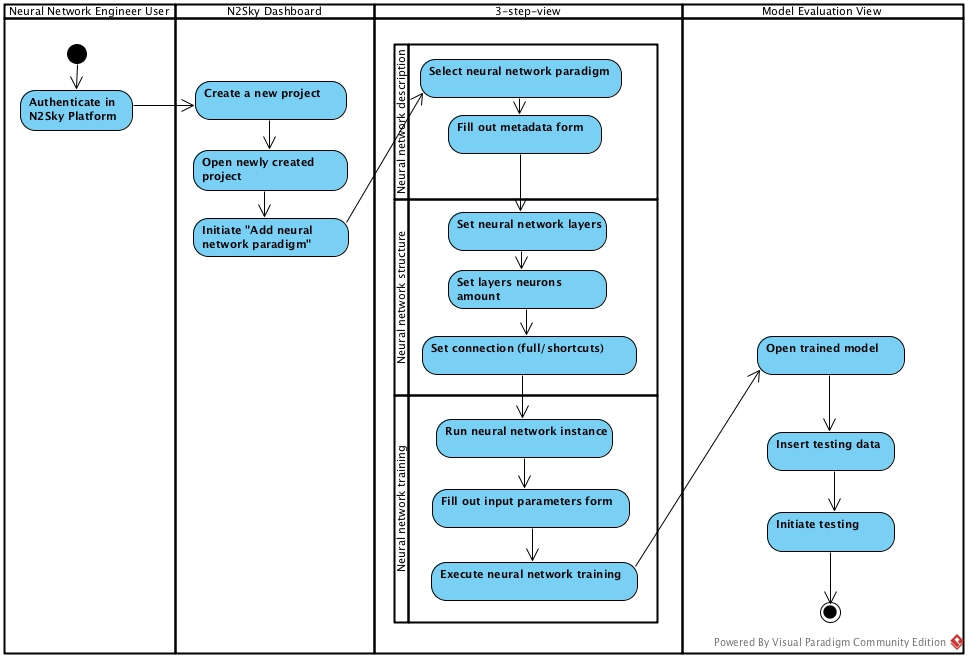
\includegraphics[width=\linewidth]{components/tutorial/img/tutorial_engeneer.jpg}
  \caption{Tutorial. Activity Diagram of creation the neural network from the existing paradigm}
  \label{fig:tutorial_engeneer}
\end{center}
\end{figure} 



Every participant is represented as a pool of activities. The following steps the user has to proceed:


\begin{itemize}
\item \emph{The neural network engineer user} 
\begin{itemize}
\item \emph{Authenticate in N2Sky platform} is the same step as by the arbitrary user.
\end{itemize}
\item \emph{N2Sky dashboard.} Create the project and open newly created project activities are the same as in the previous tutorial with the arbitrary user. Only one difference, that by choosing tool the user chooses "Add neural network paradigm".  
\item \emph{3-step-vew} is the simplified way of creation of the neural network from the paradigm. The following tabs and activities are represented:
\begin{itemize}
\item \emph{Neural network description} the first tab what user see after redirecting to the page from the project. 
\begin{itemize}
\item \emph{Select neural network paradigm.} The user can choose available paradigm from the list. After he selecting one the form with metadata will be loaded.
\item \emph{Fill out metadata form.} The form is loaded by reflection parameters from the ViNNSL template. The user needs to follow the fields with possible values and choose one in each. 
\end{itemize}
\item \emph{Neural network structure} The second tab of the "3-steps-view" after user clicking "Next" button.
\begin{itemize}
\item \emph{Set neural network layers.} The user will see three layers: the input layer, hidden layer, and output layer. Every layer can be single except hidden layer. The user can choose the amount of the hidden layers.
\item \emph{Set layers neurons amount.} After choosing the layers, the user has to type how many nodes will be in each layer. After typing it the graphical representation will appear.
\item \emph{Set connection (full/shortcuts).} There are three buttons are available: 
\begin{itemize}
\item Execute full connection, which will make the fully connected neural network between all nodes.
\item Pure shortcut, which will remove the full connection and replace it with the shortcut.
\item Only shortcut, which will leave full connection and additionally add the shortcut.
\end{itemize}

The user can choose multiple possibilities and make absolutely customized neural network structure.

\end{itemize}
\item \emph{Neural network training} the last and the most important tabs of the "3-step-view". From this tab, the user can perform training and manipulate neural network instance.
\begin{itemize}
\item \emph{Run neural network instance.} The user clicks on "Run neural network" and the popup modal window will appear. It is possible to choose the N2Sky cloud or own cloud. The engineer user does not have own cloud and he chooses N2Sky cloud. After it the neural network instance is spawning on the N2Sky cloud.
\item \emph{Fill out parameters form.} Almost the same step as by the arbitrary user, except the engineer user, does not use the default values, but type everything by himself.
\item \emph{Execute neural network training.} The user performs training with his own training data, which he has uploaded on the N2Sky platform.
\end{itemize}
\end{itemize}
 \item \emph{Model Evaluation View.} The same step as in the previous tutorial, but in this case, the user uses own testing date form evaluating the trained model.
\end{itemize}



\subsection{Upload Own Neural Network Paradigm}\label{Upload own neural network paradigm}

This tutorial is related to contributor user, which has long-term experience with neural network field and want to test his own projects on the N2Sky platform.
Some steps are common as by arbitrary and neural network engineer user, but interaction with the N2Sky platform is different.


The activity diagram, which displayed in figure \ref{fig:tutorial_contribut}, shows typical workflow of uploading own neural network paradigm. There are four main components of the diagram, which are participating in this workflow: 
\begin{enumerate}
\item The contributor user
\item N2Sky Dashboard
\item Neural network training (the last step of the "3-step-view")
\item Model Evaluation View
\end{enumerate}

\begin{figure}[htbp]
\begin{center}
  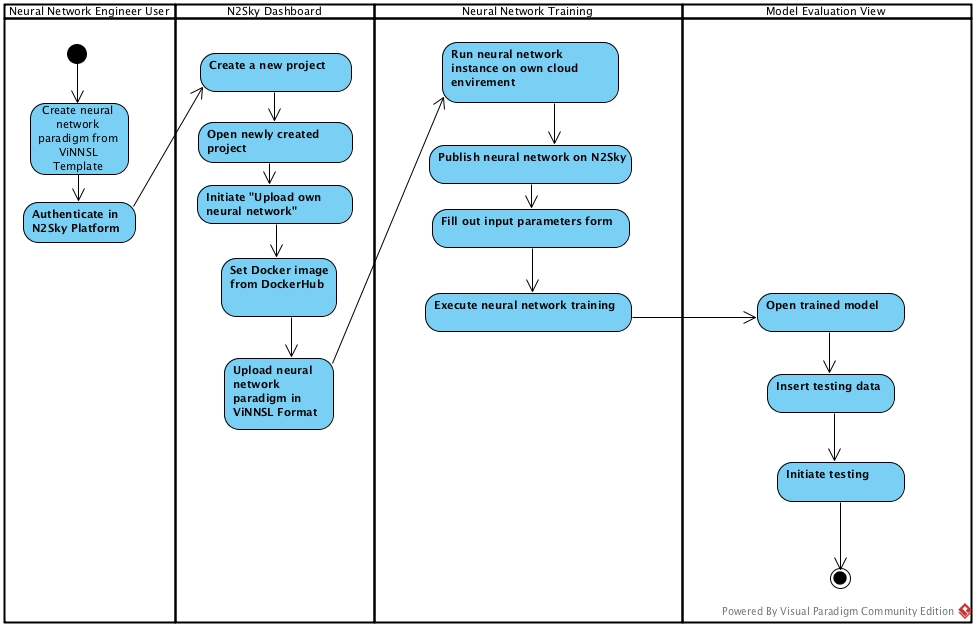
\includegraphics[width=\linewidth]{components/tutorial/img/tutorial_contribut.jpg}
  \caption{Tutorial. Activity Diagram of upload own neural network paradigm}
  \label{fig:tutorial_contribut}
\end{center}
\end{figure} 


\begin{itemize}
\item \emph{The contributor user} 
\begin{itemize}
\item \emph{Create neural network paradigm from the ViNNSL template.} This is predefinition step, which contributor user has to make before starting the workflow. How to make own ViNNSL description is described in \autoref{ViNNSL 2.0 extended}.
\item \emph{Authenticate in N2Sky platform} is the same step as by the arbitrary user.
\end{itemize}
\item \emph{N2Sky Dashboard.} The creating new project and open it are the same activities as it was described in previous tutorials. The following new steps the user has to make:
\begin{itemize}
\item \emph{Initiate "Upload own neural network"}, which will open the popup window where the user can fill out the form.
\item \emph{Set Docker imaged from the DockerHub} since the contributor user uploads own neural network, he has to push it on DockerHub repository. The N2Sky platform finds this image by DockerHub username and the image name.
\item \emph{Upload neural network paradigm in ViNNSL format}. The user uploads to N2Sky platform his neural network either in ViNNSL XML or in ViNNSL JSON. After uploading it, the user can overview and even edit his description.
\end{itemize}
\item \emph{Neural Network Training.} The last tab of the "3-step-view", which allow the user to perform training and manipulate the neural network instance.
\begin{itemize}
\item \emph{Run neural network instance on own cloud environment.} The similar as by neural network engineer user, except the contributor user, will run the instance in his own environment. Another word, the instance is already running on contributor's cloud, the user just needs to set host and endpoints to the N2Sky platform.
\item \emph{Publish neural network on N2Sky} the user can publish neural network on N2Sky by pressing "publish" button. In this case, the neural network will be available in neural network repository and other users can use it.
\item \emph{Execute neural network training.} The similar procedure as by engineer user. The contributor user uses his own training data.
\end{itemize}
\item \emph{Model Evaluation View.} The same step as by the previous tutorial, except that the user as the neural network owner can see the trained models from other users.

\end{itemize}

